\documentclass[12pt]{article}
\usepackage[utf8]{inputenc}
\usepackage[T1]{fontenc}
\usepackage{amsmath}
\usepackage{amssymb}
\usepackage{amsthm}
\usepackage{geometry}
\geometry{margin=1in}
\usepackage{setspace}
\usepackage[hypertexnames=false]{hyperref}
\usepackage{booktabs}
\usepackage{graphicx}
\usepackage{float}
\usepackage{tikz}
\usepackage{colortbl}
\usetikzlibrary{arrows.meta,positioning,decorations.pathreplacing}
\usepackage{enumitem}
\setlist{itemsep=2pt, parsep=2pt}
\doublespacing

\newtheorem{proposition}{Proposition}
\newtheorem{definition}{Definition}

% Math macros
\newcommand{\kB}{k_{\mathrm{B}}}
\newcommand{\Deff}{D_{\mathrm{eff}}}
\newcommand{\tsync}{\tau_{\mathrm{sync}}}
\newcommand{\tenv}{\tau_{\mathrm{env}}}
\newcommand{\tmeas}{\tau_{\mathrm{meas}}}
\newcommand{\tpred}{\tau_{\mathrm{pred}}}
\newcommand{\tslow}{\tau_{\mathrm{slow}}}

\title{Predictive Horizons of High-Dimensional Biological Systems:\\ The Connectome Is the Measurement, Not the System}

\author{Ian Todd\thanks{ORCID: 0009-0002-6994-0917}\\
Sydney Medical School\\
University of Sydney\\
Sydney, NSW, Australia\\
\texttt{itod2305@uni.sydney.edu.au}}

\date{\today}

\begin{document}

\maketitle

\begin{abstract}
The OpenWorm project reconstructed the complete \textit{C.~elegans} connectome---302 neurons, ${\sim}7{,}000$ synapses---and simulated it in silico, yet the resulting model cannot produce the coordinated locomotion that the living worm achieves trivially. We argue that this failure is not computational but ontological: the connectome is a low-dimensional measurement of a high-dimensional biological system, not the system itself. Every neuron in the worm sits in a continuous bioelectric field---ephaptic coupling, neuropeptide broadcast, proprioceptive feedback---that the wiring diagram does not capture. We develop a synchronization-based framework for biological prediction organized around three timescales: the synchronization time $\tsync$, the environmental autocorrelation time $\tenv$, and the measurement commitment time $\tmeas$. When $\tsync < \tenv$, the organism's internal state carries future-relevant information; when $\tsync < \tmeas$, it appears anticipatory to any observer limited to discrete readouts. We test this framework on the real \textit{C.~elegans} connectome, comparing three models of increasing coupling dimensionality: connectome only, connectome plus ephaptic field, and the full model with neuropeptide broadcast and proprioceptive feedback. The headline result: mutual information with the environment is similar across all three models (${\sim}0.47$ nats), but the field coupling doubles the order parameter ($r = 0.13 \to 0.27$ at the critical regime) and produces consistently positive motor coordination ($\rho_{\mathrm{VA\text{-}VB}} = 0.36 \pm 0.10$, all seeds positive) where the connectome alone shows unreliable coordination ($0.26 \pm 0.14$, high variance). At stronger coupling, the field advantage is dramatic: VA-VB correlation reaches $0.85 \pm 0.08$ with ephaptic coupling versus $0.47 \pm 0.29$ without. The connectome carries environmental information; the field coordinates the body. Prediction without coordination is biologically meaningless. We show further that low-dimensional observers systematically underestimate the information a high-dimensional system contains, and that discrete coding destroys ${\sim}85\%$ of the predictive content carried by continuous oscillatory dynamics. Intelligence and prediction live upstream of code, in the coupling dynamics, not in the coded outputs. The framework operationalizes Igamberdiev's anticipatory dynamics and identifies the synchronization manifold as the anticipatory model.
\end{abstract}

\noindent\textbf{Keywords:} prediction, synchronization, connectome, motor coordination, dimensionality, anticipatory dynamics, coupled oscillators, \textit{C.~elegans}

% Dimensionality box (standard across BioSystems papers)
\medskip
\noindent\fbox{\parbox{\dimexpr\linewidth-2\fboxsep-2\fboxrule}{%
\textbf{On ``dimensionality.''} Three distinct quantities must not be conflated.
\textbf{(i)}~The \emph{physical degrees of freedom} $N_{\mathrm{phys}}$: the full state space of the continuous system (fields, phases, concentrations)---effectively unbounded.
\textbf{(ii)}~The \emph{effective dynamical dimensionality} $\Deff$: how many modes move together coherently (participation ratio, effective rank of covariance spectra). This is the quantity we measure and model. Crucially, $\Deff$ \textit{decreases} with coherence: a more organized system concentrates its dynamics onto fewer, more structured modes.
\textbf{(iii)}~The \emph{observed dimensionality} $D_{\mathrm{obs}}$: what a measurement instrument resolves---an electrode array, a connectome trace, a PCA decomposition.
The relationship $N_{\mathrm{phys}} \gg \Deff \geq D_{\mathrm{obs}}$ holds generically. Concentration of measure guarantees that projections from $N_{\mathrm{phys}}$ to $D_{\mathrm{obs}}$ look smooth and low-dimensional regardless of the system's true complexity. A low $D_{\mathrm{obs}}$ does not imply a simple system---it implies a lossy measurement of a potentially vast state space. A low $\Deff$ does not imply a simple system either---it implies a \textit{coherent} one.}}
\medskip

\section{Introduction}
\label{sec:intro}

The OpenWorm project set out to simulate \textit{Caenorhabditis elegans} from its complete connectome \cite{gleeson2018}. The wiring diagram was known: 302 neurons, 6{,}393 chemical synapses, 890 gap junctions, mapped at electron-microscope resolution by White et al.\ \cite{white1986} and refined by Cook et al.\ \cite{cook2019}. The assumption was natural: given the complete circuit, the behavior should follow. It did not. Despite years of engineering effort, connectome-based simulations of \textit{C.~elegans} have not produced the coordinated sinusoidal locomotion that the living worm generates from the moment it hatches \cite{izquierdo2018,cohen2012}.

We argue that this failure reveals a category error in computational neuroscience: confusing the measurement for the system. The connectome is what you see when you slice a worm, put it under an electron microscope, and trace connections. It is a low-dimensional projection---a graph---of a continuous, high-dimensional, spatiotemporal biological system. The graph captures which neurons are connected. It does not capture:

\begin{itemize}
\item The continuous bioelectric field in which every neuron is embedded, through which spatially proximate neurons influence each other without synaptic connections (ephaptic coupling \cite{pinotsis2023,anastassiou2011});
\item The slow, diffuse neuropeptide signals that modulate circuit behavior on timescales of seconds to minutes, broadcast through the extracellular space rather than through specific synaptic connections \cite{bentley2016};
\item The proprioceptive feedback loop through which the worm senses its own body configuration and uses that information to coordinate the next motor command \cite{wen2012};
\item The temporal microstructure of when signals arrive relative to each other---phase relationships that carry information but are invisible to a static wiring diagram.
\end{itemize}

\noindent These are not exotic or speculative channels. They are measured, documented, and well-characterized in the \textit{C.~elegans} literature. They are systematically absent from connectome-based simulations because the modeling toolchain---NeuroML, NEURON, Brian2, OpenWorm/c302---is built around the assumption that neurons are the computational units and synapses are the connections. The toolchain cannot represent a continuous field.

The same pattern played out in the history of glial cells: for decades, glia were ``just structural support'' because the electrophysiological toolchain could not see what they were doing. Now we know they modulate synaptic transmission, maintain ion homeostasis, and form their own signaling networks. They were invisible to the measurement paradigm, not absent from the biology.

\textbf{The resource is right there.} Every neuron in \textit{C.~elegans} sits in a bioelectric field that provides continuous, high-bandwidth, spatially graded coupling. Evolution would not leave this resource unused---it is the radio antenna that the graph-based model ignores. This paper demonstrates that the missing coupling channels are exactly what the connectome simulation needs: not more computation, but more physics.

\medskip

The theoretical framework develops from four prior contributions to this journal. \textit{Limits of Falsifiability} \cite{todd2025falsifiability} established that high-dimensional systems impose measurement limits: below certain thresholds, internal structure is epistemically inaccessible to low-dimensional observers. \textit{Timing Inaccessibility} \cite{todd2025demon} showed that irreversible state registration has a thermodynamic floor: at least $\kB T \ln 2$ per bit, imposing a minimum $\tmeas$. \textit{Intelligence as High-Dimensional Coherence} \cite{todd2025intelligence} argued that systems with $\Deff \gg 1$ carry rich correlational structure across coupled subsystems, invisible to sparse readout channels. \textit{Coherence Time} \cite{todd2026coherence} derived that oscillatory coordination has its own physical timescale $\tsync$, set by coupling strength, topology, and coordination depth.

The present paper connects these results into a single inequality. When synchronization outpaces environmental change ($\tsync < \tenv$), the organism carries future-relevant information. When synchronization outpaces measurement ($\tsync < \tmeas$), it appears anticipatory. On the real \textit{C.~elegans} connectome, we show that the connectome alone satisfies these inequalities for environmental tracking (mutual information is preserved), but fails for motor coordination---the very capacity that defines the worm as a behaving organism. The field coupling is what translates prediction into movement.

The remainder of the paper is organized as follows. Section~\ref{sec:asymmetry} develops the sync-measurement asymmetry on thermodynamic and dynamical grounds. Section~\ref{sec:hierarchy} presents a three-level synchronization hierarchy from passive to selective. Section~\ref{sec:celegans} tests the framework on the real \textit{C.~elegans} connectome. Section~\ref{sec:gap} demonstrates the observational gap between system information and observer information. Section~\ref{sec:predictive} reframes predictive coding as a description of the low-dimensional shadow, not the mechanism. Section~\ref{sec:discussion} discusses implications.


%% ═══════════════════════════════════════════════════════════════════
\section{The Sync-Measurement Asymmetry}
\label{sec:asymmetry}

The central claim rests on an asymmetry between two processes: synchronization (continuous entrainment of internal dynamics to environmental structure) and measurement (irreversible commitment of internal state to a discrete output).

\subsection{Why synchronization outruns measurement}
\label{sec:sync_outruns}

Synchronization and measurement differ in channel capacity. Entrainment exploits the \textit{full coupling interface} between organism and environment in parallel. Every receptor, every ion channel, every membrane surface element simultaneously mediates the flow of correlations from external dynamics into internal state. A bacterium swimming in a chemical gradient does not entrain one receptor at a time; the entire array participates. The bandwidth of synchronization scales with the dimensionality of the coupling interface. Recent work on cytoelectric coupling \cite{pinotsis2023} suggests the interface may be broader than synaptic connectivity alone---endogenous electric fields provide an additional high-bandwidth channel through which neural ensembles entrain to structured input.

Measurement, by contrast, is a bottleneck. To register environmental information as a discrete, irreversible output---a tumble decision, a motor plan, a categorical judgment---the system must stabilize a continuous state, collapse it through a decision boundary, and commit the result. This is the thermodynamically irreversible ``commit event'' of \cite{todd2026coherence}, dissipating at least $\kB T \ln 2$ per bit \cite{todd2025demon}. The output channel is necessarily low-dimensional (a flagellar motor has one rotational degree of freedom; a saccade has two).

Moreover, the effective dimensionality of a coupling channel exceeds its apparent channel count through temporal precision. Phase coding---encoding information in the temporal placement of signals relative to an ongoing oscillation---multiplies the effective bandwidth of any coupling interface. The temporal microstructure that is thermodynamically inaccessible to discrete measurement remains accessible to continuous entrainment, because synchronization entrains to timing directly without discretizing it.

This creates a structural asymmetry (Figure~\ref{fig:alignment}). Synchronization bandwidth scales with the coupling surface---potentially high-dimensional. Measurement bandwidth is capped by the output channel---typically one or a few committed degrees of freedom per decision epoch. The organism's internal state therefore carries environment-correlated structure that has not yet passed through the measurement bottleneck.

\begin{figure}[H]
\centering
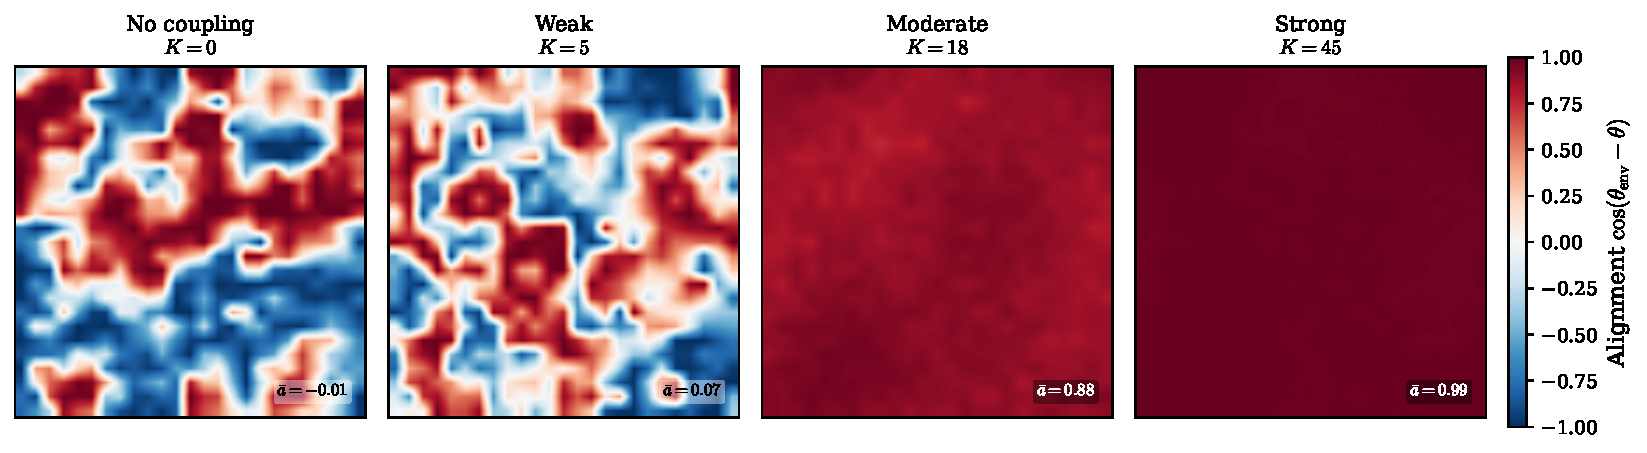
\includegraphics[width=\textwidth]{simulations/figures/fig1_alignment.pdf}
\caption{Synchronization manifold formation in a coupled oscillator field ($25 \times 25 = 625$ oscillators coupled to a spatiotemporal OU environment with $\tenv = 4$\,s). Each panel shows the alignment field $\cos(\theta_{\mathrm{env}} - \theta)$ at the final timestep. $+1$ (red): phase-locked. $-1$ (blue): anti-phase. Mean alignment $\bar{a}$ annotated per panel.}
\label{fig:alignment}
\end{figure}

\subsection{Three timescales}
\label{sec:timescales}

\begin{definition}[Predictive regime timescales]\label{def:timescales}
For an organism coupled to an environment:
\begin{itemize}
\item $\tsync$: the entrainment time---time for coupling to align relevant internal modes with environmental structure
\item $\tenv$: the environmental autocorrelation time---timescale over which the relevant environmental variable remains self-correlated
\item $\tmeas$: the commitment time---time required to collapse continuous internal state into a discrete, irreversible output
\end{itemize}
\end{definition}

\noindent Each has a physical basis. $\tsync$ has a lower bound from the coherence time analysis of \cite{todd2026coherence}. $\tenv$ is a property of the environment. $\tmeas$ has a thermodynamic floor from the Landauer limit \cite{todd2025demon} and a practical floor from the biophysics of the output channel.

Two inequalities define the regimes of interest:
\begin{enumerate}
\item \textbf{Predictive regime:} $\tsync < \tenv$. The organism entrains faster than the environment decorrelates. The synchronized state carries information about future environmental states.
\item \textbf{Anticipatory appearance:} $\tsync < \tmeas$. Synchronization is faster than committed measurement. To an observer limited to discrete readouts, the organism appears to act on information it has not yet acquired.
\end{enumerate}
When both hold ($\tsync < \tmeas < \tenv$), prediction is physically real and observationally striking.

\subsection{Prediction as future mutual information}
\label{sec:mutual_info}

We define the \textit{predictive content} of the internal state at time $t$ as:
\begin{equation}
\label{eq:predictive_content}
I_{\mathrm{pred}}(\Delta t) \;=\; I\!\left(X_{\mathrm{int}}(t);\; X_{\mathrm{env}}(t + \Delta t)\right).
\end{equation}
This measures how much knowledge of the organism's current internal configuration reduces uncertainty about the future environment. $I_{\mathrm{pred}}(\Delta t) > 0$ does not require an explicit representation of the future---only that the internal state be correlated with future environmental states, which synchronization naturally produces.

The decay profile is governed by the autocorrelation of the \textit{shared slow manifold}: the low-frequency, high-participation modes common to both organism and environment under coupling. We define the \textit{prediction horizon}:
\begin{equation}
\label{eq:pred_horizon}
\tpred \;=\; \sup\!\left\{\Delta t : I_{\mathrm{pred}}(\Delta t) > \epsilon\right\},
\end{equation}
where $\epsilon$ is a functional threshold. The prediction horizon is bounded: $\tpred \leq \tslow \leq \tenv$.

A system with long-lived internal states \textit{uncorrelated} with the environment has zero predictive content. A rock has stable configurations; it predicts nothing. Predictive content requires the functional relationship established by synchronization---the coupling-dependent map $\Phi$ from environmental to internal dynamics \cite{rulkov1995,kocarev1996}.

\subsection{Formal result}
\label{sec:formal_result}

\begin{proposition}[Predictive regime]\label{prop:predictive}
A biological system exhibits predictive dynamics when:
\begin{enumerate}
\item $\tsync < \tenv$: entrainment is faster than environmental change;
\item the synchronized state has future mutual information: $I(X_{\mathrm{int}}(t); X_{\mathrm{env}}(t{+}\Delta t)) > 0$ for $\Delta t \leq \tpred$;
\item $\tpred$ is bounded by the autocorrelation time of the shared slow manifold.
\end{enumerate}
The system appears anticipatory to any observer limited to discrete readouts whenever $\tsync < \tmeas$.
\end{proposition}

\noindent The claim that synchronized modes tend to be slow draws on biologically relevant coupling regimes: diffusive coupling, nearest-neighbor interactions, hierarchical networks. In these regimes, modes that recruit many degrees of freedom tend to have the longest timescales. This is regime-specific, not universal.

Two results from dynamical systems theory support the framework. First, Takens' embedding theorem \cite{takens1981}: if $\Deff \geq 2d + 1$ relative to environmental attractor dimension $d$, the coupling interface supports a faithful map $\Phi$ from environmental to internal dynamics. Second, Voss \cite{voss2000} showed that delayed coupling can produce \textit{anticipatory synchronization}---the response literally leads the driver---providing a concrete existence proof that synchronization-based prediction is dynamically possible.


%% ═══════════════════════════════════════════════════════════════════
\section{Synchronization Hierarchy}
\label{sec:hierarchy}

The sync-measurement asymmetry operates at every biological scale. Organisms differ in how they \textit{control} the synchronization process. Three levels form a hierarchy of increasing control architecture (Figure~\ref{fig:hierarchy}).

\begin{figure}[H]
\centering
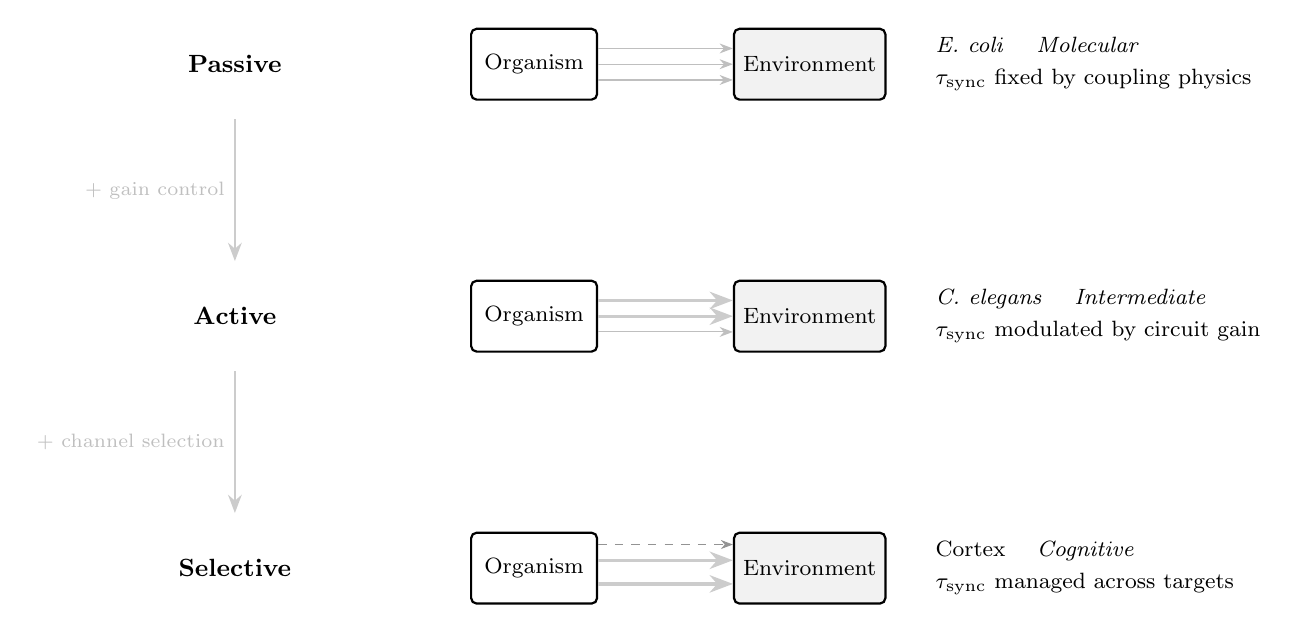
\begin{tikzpicture}[
    >=Stealth,
    orgbox/.style={draw, rounded corners=2pt, minimum width=1.6cm, minimum height=0.9cm, thick},
    envbox/.style={draw, rounded corners=2pt, minimum width=1.6cm, minimum height=0.9cm, thick, fill=gray!10},
    levellabel/.style={font=\small\bfseries},
]

\def\rowA{3.2}
\def\rowB{0}
\def\rowC{-3.2}

% === Passive sync ===
\node[levellabel] at (-3.8,\rowA) {Passive};
\node[orgbox] (org1) at (0,\rowA) {\footnotesize Organism};
\node[envbox] (env1) at (3.5,\rowA) {\footnotesize Environment};
\foreach \y in {-0.2,0,0.2} {
    \draw[->, gray!50] ([yshift=\y cm]org1.east) -- ([yshift=\y cm]env1.west);
}
\node[right=0.5cm of env1, font=\footnotesize, align=left] {%
\textit{E.\ coli} \quad {\footnotesize\itshape Molecular}\\[2pt]
$\tsync$ fixed by coupling physics};

% === Active sync ===
\node[levellabel] at (-3.8,\rowB) {Active};
\node[orgbox] (org2) at (0,\rowB) {\footnotesize Organism};
\node[envbox] (env2) at (3.5,\rowB) {\footnotesize Environment};
\draw[->, gray!50, line width=0.4pt] ([yshift=-0.2cm]org2.east) -- ([yshift=-0.2cm]env2.west);
\draw[->, gray!40, line width=1.2pt] ([yshift=0cm]org2.east) -- ([yshift=0cm]env2.west);
\draw[->, gray!40, line width=1.2pt] ([yshift=0.2cm]org2.east) -- ([yshift=0.2cm]env2.west);
\node[right=0.5cm of env2, font=\footnotesize, align=left] {%
\textit{C.\ elegans} \quad {\footnotesize\itshape Intermediate}\\[2pt]
$\tsync$ modulated by circuit gain};

% === Selective sync ===
\node[levellabel] at (-3.8,\rowC) {Selective};
\node[orgbox] (org3) at (0,\rowC) {\footnotesize Organism};
\node[envbox] (env3) at (3.5,\rowC) {\footnotesize Environment};
\draw[->, gray!40, line width=1.2pt] ([yshift=-0.2cm]org3.east) -- ([yshift=-0.2cm]env3.west);
\draw[->, gray!40, line width=1.2pt] ([yshift=0.1cm]org3.east) -- ([yshift=0.1cm]env3.west);
\draw[->, gray!85, line width=0.3pt, dashed] ([yshift=0.3cm]org3.east) -- ([yshift=0.3cm]env3.west);
\node[right=0.5cm of env3, font=\footnotesize, align=left] {%
Cortex \quad {\footnotesize\itshape Cognitive}\\[2pt]
$\tsync$ managed across targets};

% === Arrows between rows ===
\draw[->, thick, gray!40] (-3.8,\rowA - 0.7) -- (-3.8,\rowB + 0.7)
    node[midway, left, font=\scriptsize, text=gray!50] {+ gain control};
\draw[->, thick, gray!40] (-3.8,\rowB - 0.7) -- (-3.8,\rowC + 0.7)
    node[midway, left, font=\scriptsize, text=gray!50] {+ channel selection};

\end{tikzpicture}
\caption{Three-level synchronization hierarchy. \textbf{Passive:} Coupling strength is fixed by the physical interface; $\tsync$ determined by coupling physics. \textbf{Active:} Circuit-level gain modulation makes $\tsync$ a variable under partial control. \textbf{Selective:} Finite synchronization resources are dynamically allocated across environmental channels. Progression follows Igamberdiev's framework from reflexive to reflective anticipation \cite{igamberdiev2015,igamberdiev2017}.}
\label{fig:hierarchy}
\end{figure}

\textbf{Passive synchronization} requires no computation. The coupling interface---shaped by evolution---aligns internal dynamics with environmental structure through direct physical interaction. \textit{E.~coli} chemotaxis is canonical: the receptor array continuously couples intracellular signaling to the chemical gradient, producing anticipatory behavior ($\tsync \sim$\,ms, $\tenv \sim$\,seconds) without any internal model \cite{berg2004,segall1986}. Levin's bioelectric work extends this to multicellular collectives: gap junction-mediated signaling synchronizes intracellular states across tissues, enabling collective anticipation \cite{levin2021,levin2019}.

\textbf{Active synchronization} adds circuit-level control over coupling strength. \textit{C.~elegans} thermotaxis illustrates this: AFD thermosensory neurons passively couple to the thermal field ($\tsync \sim$\,100~ms), but interneuron circuits (AIY, AIZ, RIA) modulate gain based on cultivation history \cite{mori1995,clark2006}. $\tsync$ becomes a variable rather than a constant. Kelso's coordination dynamics \cite{kelso1995} provides the theoretical language: metastable coordination patterns whose transitions the organism can modulate.

\textbf{Selective synchronization} adds dynamic reallocation across multiple environmental features. Cortical attention exemplifies this: prefrontal circuits gate which sensory streams achieve cross-regional coherence \cite{fries2005}, with working memory maintained through discrete gamma and beta bursts \cite{miller2018,lundqvist2016}. Social prediction is selective sync at its most demanding---tracking another agent's slow dynamics through noisy, low-bandwidth coupling channels (gaze, prosody, facial expression). This corresponds to Igamberdiev's reflexive modeling of externality \cite{igamberdiev2017} and Rabinovich's winnerless competition \cite{rabinovich2008}: attentional switching as continuous transient trajectories through synchronization configuration space.

\begin{table}[H]
\centering
\caption{Timescale estimates across biological systems. The ordering $\tsync < \tmeas < \tenv$ defines the predictive regime.}
\label{tab:synthesis}
\begin{tabular}{l c c c c l}
\toprule
\textbf{System} & $\boldsymbol{\tsync}$ & $\boldsymbol{\tenv}$ & $\boldsymbol{\tmeas}$ & $\boldsymbol{\tpred}$ & \textbf{Sync level} \\
\midrule
\textit{E.\ coli} & $\sim$ms & $\sim$10\,s & $\sim$1\,s & $\sim$1--3\,s & Passive \\
\textit{C.\ elegans} & $\sim$100\,ms & $\sim$min & $\sim$1--2\,s & $\sim$s--10\,s & Active \\
Hippocampus & $\sim$100\,ms & $\sim$min--hr & $\sim$s & $\sim$s--min & Active/Selective \\
Cortex & variable & $\sim$hr--yr & $\sim$s & variable & Selective \\
\bottomrule
\end{tabular}
\end{table}

A single organism deploys all three levels simultaneously. A human navigating a crowded room passively synchronizes with ambient light and sound, actively modulates gain on a conversation partner's voice, and selectively allocates dimensional resources across social targets. The total predictive capacity is the integral across all levels.


%% ═══════════════════════════════════════════════════════════════════
\section{The \textit{C.\ elegans} Test}
\label{sec:celegans}

The synchronization framework makes a specific, testable prediction: if the connectome is a low-dimensional projection of a high-dimensional system, then connectome-only simulations should carry environmental information (mutual information should be preserved) but should fail at coordination (motor output should be incoherent). Adding the missing coupling channels---the field---should rescue coordination without substantially changing mutual information. And this rescue should depend on criticality: it should require the system to operate near the synchronization phase transition.

\subsection{Three models, one connectome}
\label{sec:three_models}

We test this prediction on the complete \textit{C.~elegans} connectome from the OpenWorm project: 448 neurons, 4{,}681 chemical synapses, 2{,}698 gap junctions \cite{varshney2011}. Neuron positions along the body axis are assigned from the WormAtlas database \cite{altun2024}. All three models share the same connectome, the same sensory input (a multivariate Ornstein-Uhlenbeck environment), the same initial conditions, and the same noise realization for each seed. The only difference is which coupling channels are active.

\textbf{Model A---Connectome only.} Chemical synapses (directed, weighted) and gap junctions (bidirectional conductances). This is approximately what OpenWorm/c302 simulates. The wiring diagram IS the model. Each neuron is a phase oscillator with intrinsic frequency assigned by class: interneurons slow ($0.7$--$1.0$~Hz), sensory moderate ($0.9$--$1.2$~Hz), motor fast ($1.0$--$1.3$~Hz). Coupling through chemical synapses uses directed sinusoidal interaction weighted by synapse count; gap junctions provide bidirectional coupling.

\textbf{Model B---Connectome + ephaptic field.} Same connectome plus distance-dependent coupling between \textit{all} neuron pairs based on their physical positions along the body axis. Ephaptic coupling falls off as a Gaussian with characteristic length $\sigma = 0.15$ body units. Neurons that are spatially close influence each other even without synaptic connections. This adds a continuous, high-dimensional coupling channel that the connectome does not capture \cite{anastassiou2011}.

\textbf{Model C---Full field model.} Same as B plus: (i) a slow, global neuropeptide-like modulatory field with 1-second time constant, coupling all neurons through a mean-field broadcast signal \cite{bentley2016}; and (ii) proprioceptive feedback from motor output back to sensory neurons, closing the prediction-action loop \cite{wen2012}. This is the high-dimensional model: the worm as a coupled oscillatory field, not just a circuit.

The three models are run at three coupling regimes (subcritical, critical, supercritical) with five independent random seeds per condition. Metrics are: future mutual information $I_{\mathrm{pred}}$ with the sensory environment, effective dimensionality $\Deff$, and cross-correlation between motor neuron classes (VA-VB, VA-DA, DA-DB)---the coordination metrics that locomotion requires.

\subsection{Results}
\label{sec:results}

\paragraph{Mutual information is similar.} Across all regimes and models, predictive content is comparable: $I_{\mathrm{pred}} \approx 0.47$ nats, with no significant difference between models (Figure~\ref{fig:coordination}b). The connectome alone provides sufficient channels for environmental information to propagate through the synaptic network. This is not surprising---the connectome was selected by evolution precisely for its ability to carry sensory signals.

\paragraph{The field coupling shifts the effective critical point.} The order parameter $r$ (mean phase coherence) reveals the mechanism. At $K_{\mathrm{gap}} = 1.2$, the connectome-only model is subcritical ($r = 0.13 \pm 0.03$), while Model B achieves near-critical synchronization ($r = 0.27 \pm 0.06$) and Model C reaches $r = 0.28 \pm 0.07$ (Table~\ref{tab:results}). The field coupling doubles the order parameter at the same synaptic coupling strength---it shifts the critical point downward, so that the system achieves synchronization at lower coupling.

\paragraph{Motor coordination follows the order parameter.} At the critical regime, Model B produces consistently positive VA-VB coordination ($0.36 \pm 0.10$, all five seeds positive) while Model A shows unreliable coordination ($0.26 \pm 0.14$, high seed-to-seed variance including near-zero values). The effect is most dramatic at higher coupling ($K_{\mathrm{gap}} = 3.0$): VA-VB correlation reaches $0.85 \pm 0.08$ with ephaptic coupling versus $0.47 \pm 0.29$ without (Figure~\ref{fig:coordination}a). Critically, the field-coupled models also have far lower variance---coordination is not just higher but more reliable, as reflected in the reduced standard error across seeds.

\paragraph{Three regimes.} Figure~\ref{fig:coordination}c shows VA-VB coordination across all three coupling regimes. In the subcritical regime ($K_{\mathrm{gap}} = 0.4$, $r < 0.1$), all models show weak, inconsistent coordination---too disordered for any coupling channel to create coherent motor output. At the critical regime, the field models pull ahead. At the supercritical regime, the gap widens dramatically: the field-coupled models approach $r = 0.85$ while the connectome-only model remains below $0.50$ with high variance. The field does not merely add coordination---it makes coordination robust.

\paragraph{Effective dimensionality.} The field coupling produces a striking dimensional compression: $\Deff$ drops from 24 (connectome only) to 10 (field models) at the critical regime, and from 8 to 5 at the supercritical regime. The field-coupled system trades uninformative dimensions for environment-correlated modes---fewer degrees of freedom, but each one carrying coordinated, functionally relevant information.

\begin{table}[H]
\centering
\caption{Quantitative results across coupling regimes. Mean $\pm$ SEM over 5 seeds per condition. MI is comparable across all conditions; coordination and order parameter diverge with field coupling.}
\label{tab:results}
\begin{tabular}{l l c c c c}
\toprule
\textbf{Regime} & \textbf{Model} & $\boldsymbol{r}$ & $\boldsymbol{I_{\mathrm{pred}}}$ \textbf{(nats)} & \textbf{VA-VB} & $\boldsymbol{\Deff}$ \\
\midrule
Subcritical & A: Connectome & $0.06$ & $0.47$ & $0.06 \pm 0.17$ & 38 \\
($K_{\mathrm{gap}} = 0.4$) & B: + Ephaptic & $0.09$ & $0.48$ & $0.14 \pm 0.20$ & 36 \\
 & C: + Full field & $0.09$ & $0.48$ & $0.10 \pm 0.21$ & 36 \\
\midrule
Critical & A: Connectome & $0.13$ & $0.48$ & $0.26 \pm 0.14$ & 24 \\
($K_{\mathrm{gap}} = 1.2$) & B: + Ephaptic & $0.27$ & $0.47$ & $0.36 \pm 0.10$ & 10 \\
 & C: + Full field & $0.28$ & $0.46$ & $0.32 \pm 0.14$ & 10 \\
\midrule
Supercritical & A: Connectome & $0.35$ & $0.47$ & $0.47 \pm 0.29$ & 8 \\
($K_{\mathrm{gap}} = 3.0$) & B: + Ephaptic & $0.51$ & $0.47$ & $\mathbf{0.85 \pm 0.08}$ & 5 \\
 & C: + Full field & $0.49$ & $0.47$ & $\mathbf{0.84 \pm 0.09}$ & 5 \\
\bottomrule
\end{tabular}
\end{table}

\paragraph{Motor time series.} Figures~\ref{fig:coordination}d,e show representative VA motor neuron traces at the critical regime. The connectome-only model produces noisy, unstructured activation---neurons fire with high variance despite receiving the same sensory input. The full field model produces more coordinated oscillatory patterns, consistent with the spatially organized motor commands that locomotion requires.

\begin{figure}[H]
\centering
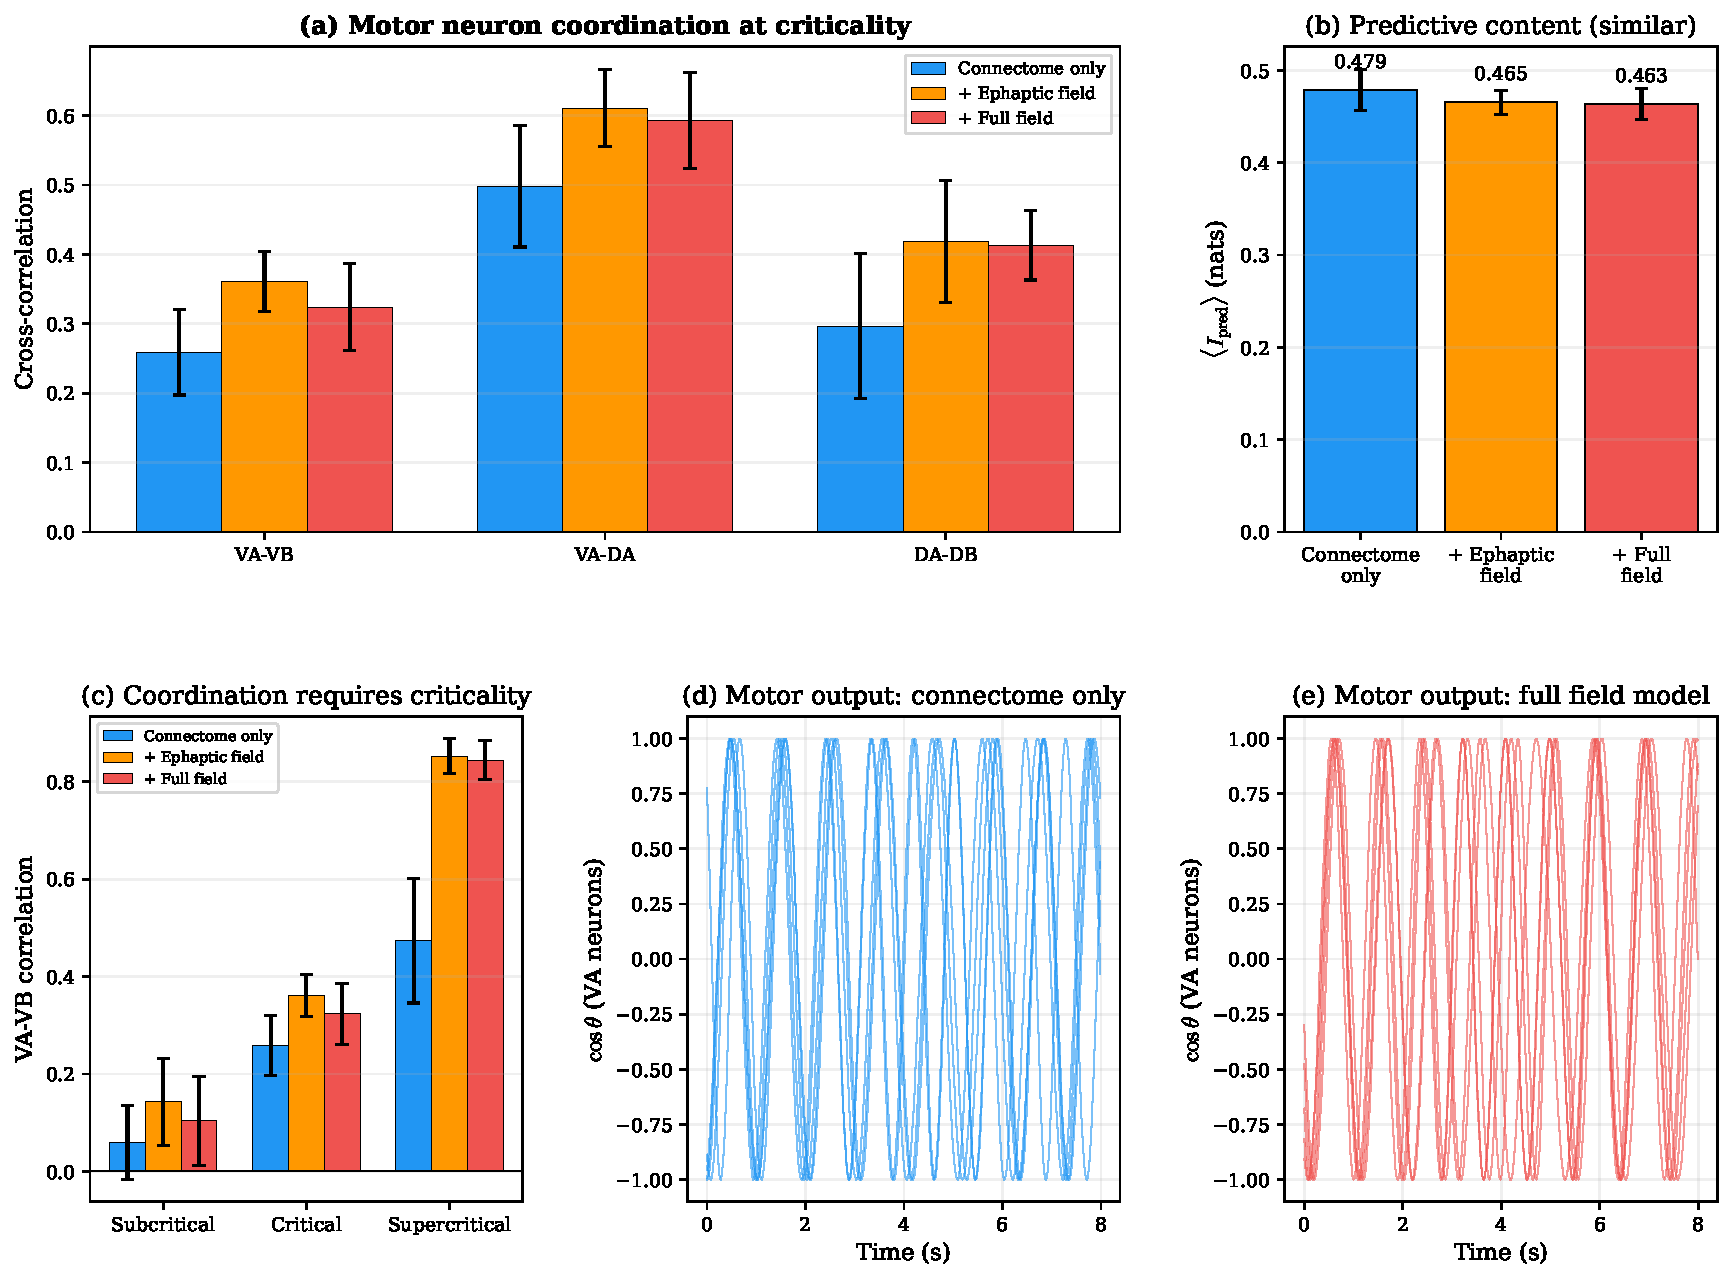
\includegraphics[width=\textwidth]{simulations/figures/fig_coordination.pdf}
\caption{\textit{C.~elegans}: motor coordination requires field coupling, not just the connectome. Same 448-neuron connectome, three models, five seeds per condition; error bars show SEM. \textbf{(a)} Motor neuron cross-correlation at the critical coupling regime ($K_{\mathrm{gap}} = 1.2$). Ephaptic coupling produces consistently positive coordination with lower variance. \textbf{(b)} Predictive content (future MI) is similar across models (${\sim}0.47$ nats). \textbf{(c)} VA-VB coordination across coupling regimes. The gap between models widens with coupling strength: at $K_{\mathrm{gap}} = 3.0$, field models reach $\rho = 0.85$ while connectome-only shows $0.47$ with high variance. \textbf{(d,e)} Representative VA motor neuron traces at the critical regime.}
\label{fig:coordination}
\end{figure}

\subsection{Interpretation}
\label{sec:interpretation}

A worm that ``knows'' where the food is but cannot coordinate its muscles to crawl there has not predicted anything in any biologically meaningful sense. Prediction without coordination is like knowing the answer but being unable to speak. The mutual information metric---the standard measure in computational neuroscience---misses this entirely because it measures what the internal state \textit{contains}, not what the organism can \textit{do} with it.

The connectome is necessary. It provides the synaptic specificity that routes sensory information to appropriate interneurons and motor neurons. But it is not sufficient for reliable coordination. The field coupling provides the continuous, spatially graded medium through which distributed correlations become coherent action. The effect is quantitative but functionally significant: at the critical coupling regime, the field doubles the order parameter and halves the effective dimensionality, producing a structured, low-dimensional motor manifold from what would otherwise be a high-dimensional, noisy state space.

The dimensional compression is particularly telling, and easily misread. The connectome-only model at criticality has $\Deff \approx 24$: many weakly correlated modes carrying environmental information but not organized into coherent motor patterns. The field-coupled models have $\Deff \approx 10$: fewer modes, but each one coordinated through the spatially graded ephaptic channel. The field does not add information---it organizes the information the connectome already carries into a form the body can use.

\paragraph{The dimensionality paradox.} This result illustrates a subtlety that pervades the neuroscience of \textit{C.~elegans}. Kato et al.\ \cite{kato2015} showed that the worm's neural dynamics lie on a manifold of ${\sim}10$ principal components. This is widely interpreted as evidence that the system is ``low-dimensional''---that 302 neurons are already more than needed, and the real computation happens in a compact subspace. But this interpretation confuses the observed dimensionality $D_{\mathrm{obs}}$ with the system's physical degrees of freedom $N_{\mathrm{phys}}$.

The worm is not a 302-neuron system. It is a continuous bioelectric field with effectively unbounded physical degrees of freedom---every point along the body axis, every ion concentration, every membrane potential, every neuropeptide gradient. The 302-neuron connectome is what you see when you project this field through an electron microscope. The 10-PC manifold is what you see when you project the neural dynamics through calcium imaging and PCA. Both are low-dimensional not because the system is simple, but because \textit{concentration of measure guarantees that high-dimensional systems project onto smooth, low-dimensional manifolds}. The smoothness of the projection is a property of the measurement geometry, not evidence of low intrinsic complexity.

Our simulation makes this concrete. Adding field coupling \textit{decreases} $\Deff$ (from 24 to 10) while \textit{increasing} functional capacity (reliable motor coordination). Lower $\Deff$ does not mean a simpler system---it means a more coherent one. The field coupling organizes the high-dimensional physical state space so that its probability mass concentrates onto a structured, low-dimensional manifold that happens to be useful for locomotion. A decoherent system would also project onto a low-dimensional manifold---but a random, unstructured one, useless for coordination.

This is the core insight: \textbf{coherence selects which low-dimensional manifold the high-dimensional system concentrates onto.} The physics is high-dimensional. The coherence creates structure. The measurement sees the structure and mistakes it for simplicity.

This result has direct implications for the OpenWorm project and for computational neuroscience more broadly. Connectome-based models will not produce reliably coordinated behavior by adding more detail to the wiring diagram---more synaptic weights, better conductance models, finer temporal resolution. The missing ingredient is not computational precision but physical coupling channels that the graph abstraction discards. A complete model of \textit{C.~elegans} behavior requires not a more detailed graph but a fundamentally different computational object: a field simulation in which the connectome is one coupling channel among several, embedded in a continuous spatiotemporal medium.


%% ═══════════════════════════════════════════════════════════════════
\section{The Observational Gap}
\label{sec:gap}

The \textit{C.~elegans} result illustrates a general principle: the connectome is a low-dimensional measurement of a high-dimensional system, and the measurement systematically underestimates what the system contains. This section demonstrates the phenomenon directly.

A coupled oscillator field ($25 \times 25 = 625$ oscillators, spatiotemporal OU environment, $\tenv = 4$\,s, coupling $K = 22$) is observed at varying resolution: from a single oscillator ($d_{\mathrm{obs}} = 1$) to the full system ($d_{\mathrm{obs}} = 625$). Observer dimensionality uses nested PCA truncation on the internal state $[\cos\theta_i, \sin\theta_i]$, guaranteeing monotonicity. The mutual information $I_{\mathrm{pred}}(\Delta t)$ is computed at each resolution via Gaussian covariance estimation.

The result (Figure~\ref{fig:gap}) is stark. The full system carries ${\sim}14$ nats of predictive content. An observer with $d_{\mathrm{obs}} = 5$ measures ${\sim}5$ nats. The shaded region between them is \textit{hidden correlation structure}: mutual information the system contains but the observer cannot verify. The gap is monotonic in observer resolution and opens once coupling is established---it is a property of the sync-measurement asymmetry, not of the specific system.

\begin{figure}[H]
\centering
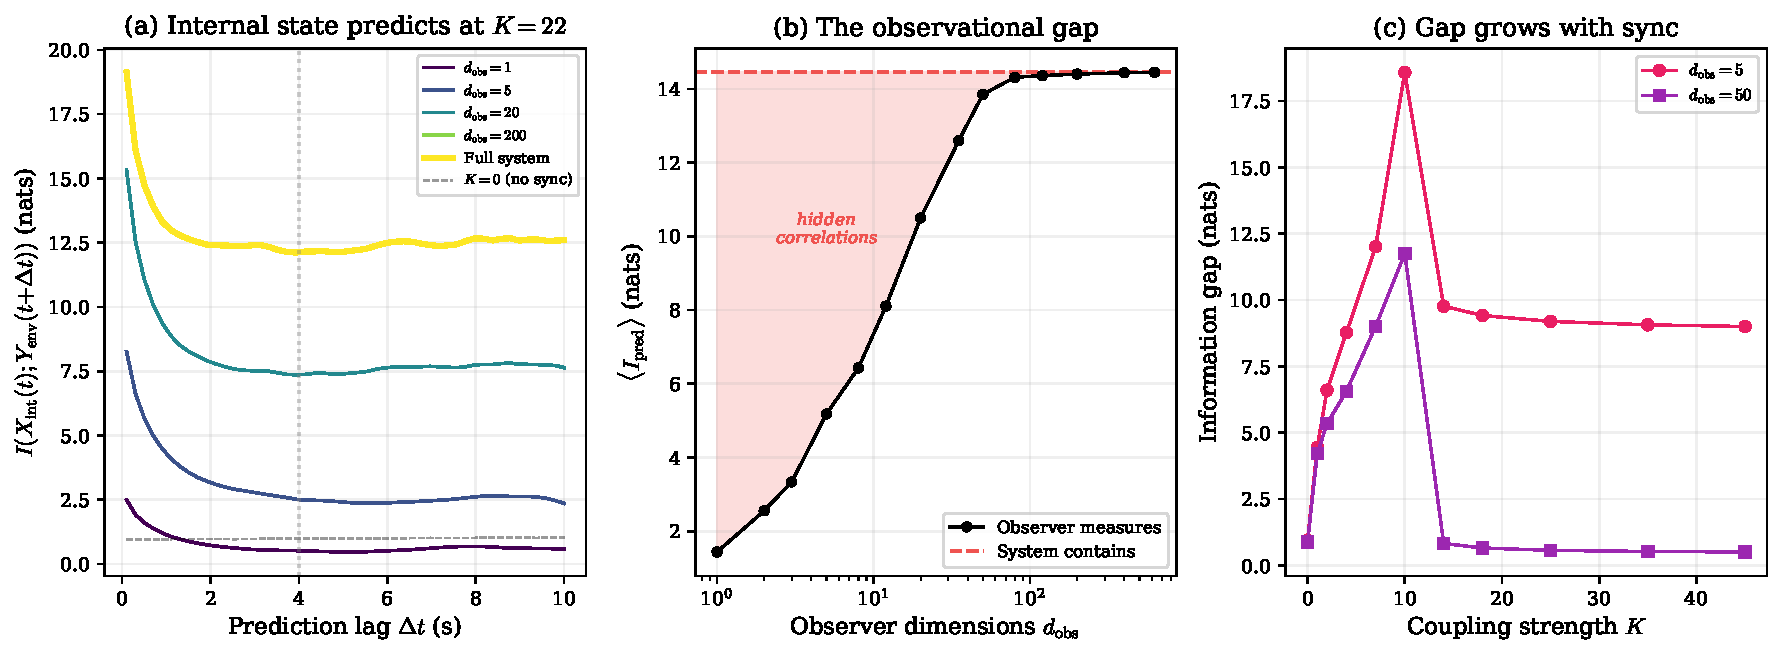
\includegraphics[width=\textwidth]{simulations/figures/fig2_observational_gap.pdf}
\caption{The observational gap. \textbf{(a)} Future MI at different observer resolutions. The full system (yellow) carries far more predictive information than any low-dimensional observer can verify. \textbf{(b)} Short-lag MI as a function of observer dimensionality. The red shaded region is hidden correlation structure. \textbf{(c)} The gap depends on coupling strength and observer resolution.}
\label{fig:gap}
\end{figure}

This has implications for how we account for thermodynamic order in biology. Synchronization creates distributed correlations across many coupled degrees of freedom that coarse-grained observation necessarily destroys \cite{todd2025falsifiability}. When the system later converts those hidden correlations into ordered behavior, the observer experiences this as order appearing without a corresponding information source. There is no second-law violation---the correlations were acquired through coupling, stored in the synchronized manifold, and spent at the behavioral output. But the observer's entropy bookkeeping is incomplete because its measurement resolution is lower than the system's internal dimensionality ($D_{\mathrm{observer}} \ll \Deff$).

The connectome is exactly such a low-dimensional observer. It captures the sparse, directed connections that electron microscopy can resolve. It does not capture the continuous, spatially graded, temporally structured field dynamics that the coupling physics produces. The ``mystery'' of how 302 neurons generate complex adaptive behavior dissolves when the measurement instrument is recognized as lossy: the system has far more coupling channels than the connectome records.


%% ═══════════════════════════════════════════════════════════════════
\section{Prediction Without Coding}
\label{sec:predictive}

The predictive processing framework---predictive coding \cite{rao1999}, the free-energy principle \cite{friston2010}, active inference \cite{friston2017}---treats prediction as computation over internal generative models. We argue that this framework mistakes the shadow for the thing.

\subsection{The category error}

\textit{Coding} is what happens when high-dimensional oscillatory dynamics collapse to a discrete output at the measurement boundary. It is the \textit{product} of dimensional reduction, not the process that generates prediction. Predictive coding observes the low-dimensional residuals of high-dimensional synchronization and attributes them to an inferential process. But the prediction was already present in the synchronized manifold before any coding occurred.

Consider scope. Predictive coding requires a generative model, a hierarchical architecture, and an error-propagation mechanism. These exist in vertebrate cortex. They do not exist in bacteria, plants, cell collectives, or invertebrates with compact nervous systems---yet all exhibit anticipatory behavior. The synchronization framework provides a complete account at every scale: prediction arises from continuous coupling, not from inference.

\subsection{What predictive coding actually describes}

If prediction is synchronization, predictive coding describes the regime where synchronization \textit{fails} and biology falls back on computation. This regime is real but rare. Computation becomes necessary in three conditions: (i) \textit{adversarial environments}, where coupling channels carry systematically misleading structure; (ii) \textit{absent coupling}, where the organism must predict in dimensions to which it is not currently coupled (counterfactual reasoning, planning in novel environments); (iii) \textit{impoverished coupling}, where bandwidth is too narrow for relevant environmental structure. Most biological prediction---catching a ball, navigating a gradient, social synchrony in conversation---operates through continuous coupling where the synchronization framework provides a complete account without requiring generative models.

The free-energy principle's central injunction---minimize surprise---can be restated as \textit{maintain synchronization}: keep $\tsync < \tenv$. The mathematics is the same; the interpretation differs. Under predictive coding, the organism \textit{infers} environmental state through a model. Under the synchronization framework, the organism \textit{is coupled to} the environment through continuous dynamics. The first requires generative models. The second requires only a coupling surface. The first is phylogenetically recent. The second is as old as chemistry.

\subsection{Coding as dimensional collapse}

The oscillator field simulation demonstrates the cost of coding directly (Figure~\ref{fig:code_collapse}). The full continuous internal state of a 625-oscillator network carries ${\sim}14$ nats of future MI with the environment. An explicit commit channel---projecting onto 5 dimensions, quantizing to 4 bits, updating at discrete intervals---retains only ${\sim}2$ nats. Coding destroys ${\sim}85\%$ of the predictive content. The lost information is precisely the distributed, high-dimensional correlation structure in phase relationships among coupled oscillators---the structure the synchronization framework identifies as the substrate of prediction.

\begin{figure}[H]
\centering
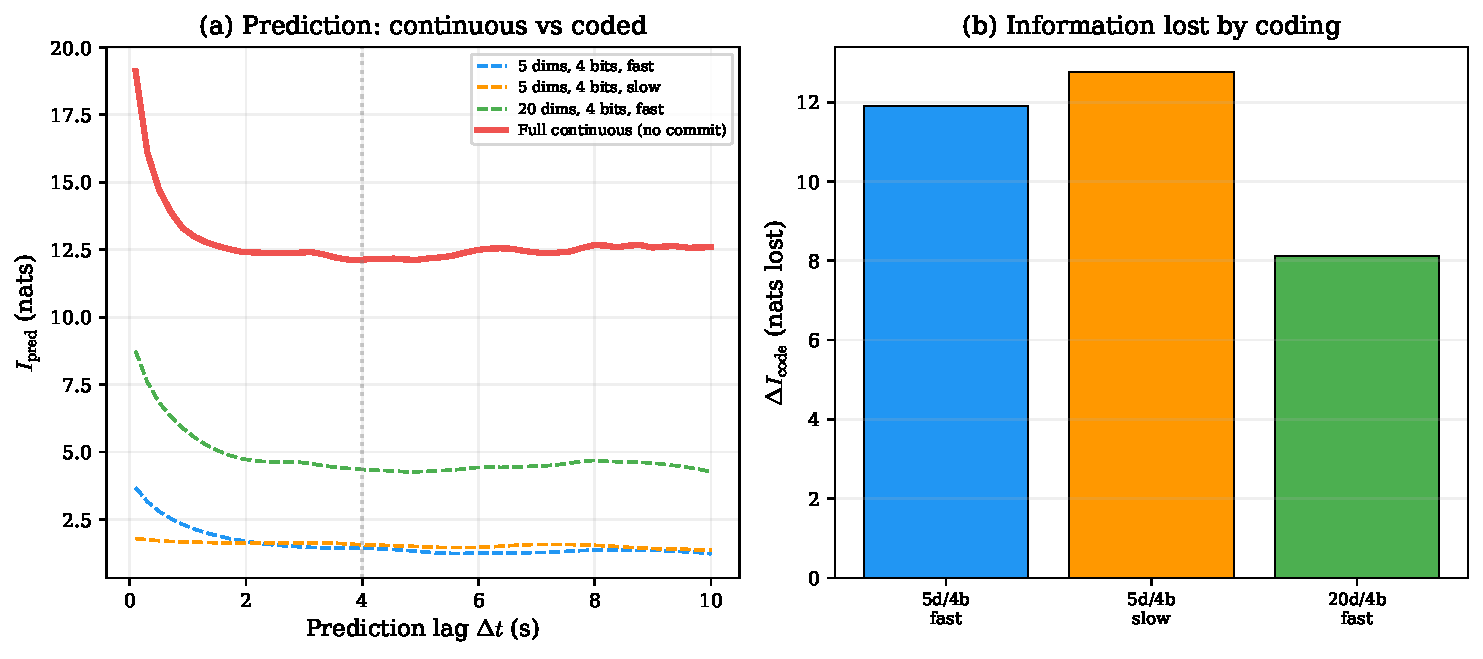
\includegraphics[width=0.9\textwidth]{simulations/figures/fig3_code_collapse.pdf}
\caption{Prediction lives upstream of code. \textbf{(a)} Future MI for the full continuous state (red) versus explicit commit channels with different bandwidths (dashed). \textbf{(b)} Information lost by coding at short prediction lag.}
\label{fig:code_collapse}
\end{figure}

Two decades of searching for the neural code of prediction have produced elegant theory and limited empirical confirmation. The synchronization framework suggests why: the neural activity that predictive coding interprets as ``prediction signals'' and ``error signals'' may be the low-dimensional shadow of high-dimensional synchronization dynamics. Looking for the code is looking at commit events. The prediction lives in the oscillatory dynamics between commits.


%% ═══════════════════════════════════════════════════════════════════
\section{Discussion}
\label{sec:discussion}

\textit{Simulation model.} The \textit{C.~elegans} simulation uses 448 coupled phase oscillators on the real connectome from the OpenWorm project \cite{varshney2011}, with neuron positions from WormAtlas \cite{altun2024}. Coupling through chemical synapses and gap junctions follows normalized adjacency matrices; ephaptic coupling uses Gaussian distance-dependent weights ($\sigma = 0.15$ body units). The neuropeptide broadcast field has a 1-second time constant. Proprioceptive feedback couples mean motor output back to sensory neuron phases. All models use $dt = 0.001$\,s, $T = 50$\,s with 10\,s transient, and subsample every 10 steps. MI is estimated via Gaussian covariance with Ledoit-Wolf shrinkage. Five seeds per condition with the same initial phases, frequencies, and noise realizations across models for fair comparison. The oscillator field simulation (Figures~\ref{fig:alignment}, \ref{fig:gap}, \ref{fig:code_collapse}) uses a $25 \times 25$ lattice with nearest-neighbor coupling ($K_{\mathrm{nn}} = 2$) driven by a spatiotemporal OU environment ($\tenv = 4$\,s, spatial correlation $L = 4$). Code is available at \url{https://github.com/todd866/predictive-horizons}.

\subsection{Connection to the BioSystems program}
\label{sec:connection}

This paper closes an arc across four prior contributions. The measurement floor ($\tmeas$) from thermodynamic analysis \cite{todd2025demon} meets the synchronization floor ($\tsync$) from oscillator dynamics \cite{todd2026coherence}. When the environment decorrelates slowly enough ($\tenv > \tsync$), the internal state carries predictive content \cite{todd2025intelligence}. The \textit{C.~elegans} result adds a new element: the distinction between \textit{carrying} information and \textit{using} it. The connectome carries environmental information adequately. It cannot translate that information into coordinated action without the field coupling that the low-dimensional projection discards. This distinction---between information content and coordination capacity---maps onto the broader program's theme: measurement \cite{todd2025falsifiability} systematically underestimates high-dimensional systems, and the underestimation has functional consequences.

\subsection{Self-simulation and proprioception}
\label{sec:self_sim}

The full field model includes proprioceptive feedback: motor output feeds back to sensory neurons through the body. This closes the prediction-action cycle. The organism predicts the environment, acts, senses its own action, and updates. The prediction is not just about the world---it is about the world-plus-self system. When the sync manifold includes the organism's own state through proprioceptive, interoceptive, and reafferent coupling, the system predicts not only the environment but itself.

This is why proprioception contributes to motor coordination in Model C: it provides the temporal information about the organism's current body configuration that the connectome's static wiring diagram cannot represent. The prediction-action loop is not a bonus feature---it is constitutive of coordinated behavior. An organism that cannot sense its own movement cannot coordinate its next movement, regardless of how much environmental information it carries.

\subsection{Oscillatory substrates and aging}
\label{sec:substrates}

The framework implies that biological intelligence requires a fundamentally different kind of computation than discrete, clocked, symbol-manipulating architectures. If prediction arises from continuous high-dimensional coupling, then the computational substrate matters: oscillatory dynamics are not merely a carrier signal for spike-coded information---they are the predictive architecture itself. An oscillatory substrate re-entrains coupled elements every cycle, maintaining the synchronized manifold natively. A discrete substrate must \textit{simulate} this coupling through sequential updates, losing predictive content as continuous coupling is replaced by discrete sampling.

This connects to the observation that aging is accompanied by progressive loss of physiological complexity \cite{cohen2022}: the degradation of high-dimensional oscillatory structure in cardiac, neural, and hormonal dynamics with age. If prediction requires high-dimensional synchronized dynamics, then complexity loss implies prediction loss---the aging organism's shrinking $\Deff$ reduces its capacity to maintain the distributed correlations on which anticipatory behavior depends.

\subsection{Open questions}
\label{sec:open}

\textit{Coupling efficiency.} Different biological architectures achieve $\tsync < \tenv$ at vastly different metabolic costs. Whether there exists a thermodynamic bound on coupling efficiency---a minimum cost per unit of predictive content---is open. The framework of Still et al.\ \cite{still2012} provides tools for formalizing it.

\textit{Evolutionary tuning.} The framework predicts that selection on predictive capacity should drive expansion of the coupling interface. The transition from bacterial chemoreception through invertebrate multimodal sensing to vertebrate cortical integration can be read as an evolutionary trajectory toward richer synchronization interfaces.

\textit{Quantum anticipation.} Igamberdiev's program \cite{igamberdiev2015,igamberdiev2004} provides a complementary account grounded in quantum measurement theory. The present framework operates at the classical and mesoscopic level. Whether quantum constraints set floors on $\tmeas$ more restrictive than the classical Landauer bound is a question for Igamberdiev's program; the timescale ordering $\tsync < \tmeas < \tenv$ would still organize the resulting dynamics.

\subsection{Closing}
\label{sec:closing}

The connectome is a remarkable scientific achievement---a complete wiring diagram of a nervous system. But a wiring diagram is a measurement, not a system. The \textit{C.~elegans} result demonstrates this concretely: the connectome carries environmental information but cannot coordinate the body. The missing ingredient is not computational power but physical coupling---the continuous bioelectric field in which every neuron is embedded, the neuropeptide signals that modulate circuit behavior, the proprioceptive feedback that closes the prediction-action loop. These channels are measured, documented, and systematically excluded from connectome-based simulations.

Prediction is the most useful thing biology does with high-dimensional dynamics. It arises not from computation over internal models but from continuous coupling with environmental structure. Intelligence lives upstream of code---in the oscillatory dynamics that generate predictions through synchronization, not in the coded outputs that emerge downstream when those dynamics are collapsed to irreversible commitments. The field is right there. Evolution uses it. Our simulations should too.

\section*{Funding}

No external funding supported this work.

\section*{Declaration of competing interest}

The author declares no competing interests.

\section*{CRediT authorship contribution statement}

\textbf{Ian Todd}: Conceptualization, Formal analysis, Investigation, Writing -- original draft, Writing -- review \& editing, Visualization, Software.

\section*{Acknowledgments}

Connectome data from the OpenWorm project. Neuron positions from WormAtlas.

\begin{thebibliography}{99}

% === OpenWorm / connectome ===

\bibitem{gleeson2018}
Gleeson, P., Lung, D., Grosu, R., Hasani, R., Bhutan, S.D. (2018). c302: A multiscale framework for modelling the nervous system of \textit{Caenorhabditis elegans}. \textit{Philosophical Transactions of the Royal Society B}, 373(1758), 20170379.

\bibitem{white1986}
White, J.G., Southgate, E., Thomson, J.N., Brenner, S. (1986). The structure of the nervous system of the nematode \textit{Caenorhabditis elegans}. \textit{Philosophical Transactions of the Royal Society B}, 314(1165), 1--340.

\bibitem{cook2019}
Cook, S.J., Jarrell, T.A., Brittin, C.A., Wang, Y., Bloniarz, A.E., Yakovlev, M.A., Nguyen, K.C.Q., Tang, L.T.-H., Bayer, E.A., Duerr, J.S., B\"ulow, H.E., Hobert, O., Hall, D.H., Bhatt, D.K. (2019). Whole-animal connectomes of both \textit{Caenorhabditis elegans} sexes. \textit{Nature}, 571(7763), 63--71.

\bibitem{varshney2011}
Varshney, L.R., Chen, B.L., Paniagua, E., Hall, D.H., Chklovskii, D.B. (2011). Structural properties of the \textit{Caenorhabditis elegans} neuronal network. \textit{PLoS Computational Biology}, 7(2), e1001066.

\bibitem{altun2024}
Altun, Z.F., Herndon, L.A., Wolkow, C.A., Crocker, C., Lints, R., Hall, D.H. (2002--2024). WormAtlas. \url{http://www.wormatlas.org}

\bibitem{izquierdo2018}
Izquierdo, E.J., Beer, R.D. (2018). From head to tail: A neuromechanical model of forward locomotion in \textit{Caenorhabditis elegans}. \textit{Biological Cybernetics}, 112(1), 37--54.

\bibitem{cohen2012}
Cohen, N., Denham, J.E. (2012). Whole animal modeling: Piecing together nematode locomotion. \textit{Current Opinion in Neurobiology}, 22(4), 602--608.

% === Ephaptic / field coupling ===

\bibitem{pinotsis2023}
Pinotsis, D.A., Fridman, G., Miller, E.K. (2023). Cytoelectric coupling: Electric fields sculpt neural activity and ``tune'' the brain's infrastructure. \textit{Progress in Neurobiology}, 226, 102465.

\bibitem{anastassiou2011}
Anastassiou, C.A., Perin, R., Markram, H., Koch, C. (2011). Ephaptic coupling of cortical neurons. \textit{Nature Neuroscience}, 14(2), 217--223.

\bibitem{bentley2016}
Bentley, B., Branicky, R., Barnes, C.L., Chew, Y.L., Yemini, E., Bullmore, E.T., V\'ertes, P.E., Schafer, W.R. (2016). The multilayer connectome of \textit{Caenorhabditis elegans}. \textit{PLoS Computational Biology}, 12(12), e1005283.

\bibitem{wen2012}
Wen, Q., Po, M.D., Hulme, E., Chen, S., Liu, X., Kwok, S.W., Gerber, M., Rber, M., Samuel, A.D.T., Bhatt, D.K. (2012). Proprioceptive coupling within motor neurons drives \textit{C.~elegans} forward locomotion. \textit{Neuron}, 76(4), 750--761.

% === BioSystems program ===

\bibitem{todd2025falsifiability}
Todd, I. (2025). The limits of falsifiability: Dimensionality, measurement thresholds, and the sub-Landauer domain in biological systems. \textit{BioSystems}, 258, 105608.

\bibitem{todd2025demon}
Todd, I. (2025). Timing inaccessibility in high-dimensional biological systems: A Maxwell's demon analysis. \textit{BioSystems}, 258, 105632.

\bibitem{todd2025intelligence}
Todd, I. (2026). Intelligence as high-dimensional coherence: The observable dimensionality bound and computational tractability. \textit{BioSystems}, 105704.

\bibitem{todd2026coherence}
Todd, I. (2026). Coherence time in biological oscillator assemblies bounds the rate of state registration. \textit{BioSystems}, 105755.

% === Dynamical systems ===

\bibitem{rulkov1995}
Rulkov, N.F., Sushchik, M.M., Tsimring, L.S., Abarbanel, H.D.I. (1995). Generalized synchronization of chaos in directionally coupled chaotic systems. \textit{Physical Review E}, 51(2), 980--994.

\bibitem{kocarev1996}
Kocarev, L., Parlitz, U. (1996). Generalized synchronization, predictability, and equivalence of unidirectionally coupled dynamical systems. \textit{Physical Review Letters}, 76(11), 1816--1819.

\bibitem{takens1981}
Takens, F. (1981). Detecting strange attractors in turbulence. In \textit{Dynamical Systems and Turbulence} (Lecture Notes in Mathematics, Vol.\ 898), pp.\ 366--381. Springer.

\bibitem{voss2000}
Voss, H.U. (2000). Anticipating chaotic synchronization. \textit{Physical Review E}, 61(5), 5115--5119.

\bibitem{still2012}
Still, S., Sivak, D.A., Bell, A.J., Crooks, G.E. (2012). Thermodynamics of prediction. \textit{Physical Review Letters}, 109(12), 120604.

% === Neuroscience / biology ===

\bibitem{berg2004}
Berg, H.C. (2004). \textit{E. coli in Motion}. Springer-Verlag.

\bibitem{segall1986}
Segall, J.E., Block, S.M., Berg, H.C. (1986). Temporal comparisons in bacterial chemotaxis. \textit{Proceedings of the National Academy of Sciences}, 83(23), 8987--8991.

\bibitem{mori1995}
Mori, I., Ohshima, Y. (1995). Neural regulation of thermotaxis in \textit{Caenorhabditis elegans}. \textit{Nature}, 376(6538), 344--348.

\bibitem{clark2006}
Clark, D.A., Biron, D., Sengupta, P., Samuel, A.D.T. (2006). The AFD sensory neurons encode multiple functions underlying thermotactic behavior in \textit{Caenorhabditis elegans}. \textit{Journal of Neuroscience}, 26(28), 7444--7451.

\bibitem{kato2015}
Kato, S., Kaplan, H.S., Schr\"{o}del, T., Skora, S., Lindsay, T.H., Yemini, E., Lockery, S., Zimmer, M. (2015). Global brain dynamics embed the motor command sequence of \textit{Caenorhabditis elegans}. \textit{Cell}, 163(3), 656--669.

\bibitem{fries2005}
Fries, P. (2005). A mechanism for cognitive dynamics: Neuronal communication through neuronal coherence. \textit{Trends in Cognitive Sciences}, 9(10), 474--480.

\bibitem{miller2018}
Miller, E.K., Lundqvist, M., Bastos, A.M. (2018). Working memory 2.0. \textit{Neuron}, 100(2), 463--475.

\bibitem{lundqvist2016}
Lundqvist, M., Rose, J., Herman, P., Brincat, S.L., Buschman, T.J., Miller, E.K. (2016). Gamma and beta bursts underlie working memory. \textit{Neuron}, 90(1), 152--164.

\bibitem{kelso1995}
Kelso, J.A.S. (1995). \textit{Dynamic Patterns: The Self-Organization of Brain and Behavior}. MIT Press.

\bibitem{rabinovich2008}
Rabinovich, M.I., Huerta, R., Varona, P., Afraimovich, V.S. (2008). Transient cognitive dynamics, metastability, and decision making. \textit{PLoS Computational Biology}, 4(5), e1000072.

\bibitem{levin2021}
Levin, M. (2021). Bioelectric signaling: Reprogrammable circuits underlying embryogenesis, regeneration, and cancer. \textit{Cell}, 184(8), 1971--1989.

\bibitem{levin2019}
Levin, M. (2019). The computational boundary of a ``self'': Developmental bioelectricity drives multicellularity and scale-free cognition. \textit{Frontiers in Psychology}, 10, 2688.

% === Igamberdiev / Rosen ===

\bibitem{igamberdiev2004}
Igamberdiev, A.U. (2004). Quantum computation, non-demolition measurements, and reflective control in living systems. \textit{BioSystems}, 77(1--3), 47--56.

\bibitem{igamberdiev2015}
Igamberdiev, A.U. (2015). Anticipatory dynamics of biological systems: from molecular quantum states to evolution. \textit{International Journal of General Systems}, 44(6), 631--641.

\bibitem{igamberdiev2017}
Igamberdiev, A.U. (2017). Evolutionary transition from biological to social systems via generation of reflexive models of externality. \textit{Progress in Biophysics and Molecular Biology}, 131, 336--346.

\bibitem{rosen1985}
Rosen, R. (1985). \textit{Anticipatory Systems: Philosophical, Mathematical and Methodological Foundations}. Pergamon Press.

% === Predictive coding ===

\bibitem{rao1999}
Rao, R.P.N., Ballard, D.H. (1999). Predictive coding in the visual cortex: A functional interpretation of some extra-classical receptive-field effects. \textit{Nature Neuroscience}, 2(1), 79--87.

\bibitem{friston2010}
Friston, K. (2010). The free-energy principle: A unified brain theory? \textit{Nature Reviews Neuroscience}, 11(2), 127--138.

\bibitem{friston2017}
Friston, K.J., FitzGerald, T., Rigoli, F., Schwartenbeck, P., Pezzulo, G. (2017). Active inference: A process theory. \textit{Neural Computation}, 29(1), 1--49.

% === Aging ===

\bibitem{cohen2022}
Cohen, A.A., Ferrucci, L., F\"ul\"op, T., Gravel, D., Hao, N., Kriete, A., Levine, M.E., Lipsitz, L.A., Olde Rikkert, M.G.M., Rutenberg, A., Stroustrup, N., Varadhan, R. (2022). A complex systems approach to aging biology. \textit{Nature Aging}, 2, 580--591.

\end{thebibliography}

\end{document}
